\documentclass[10pt, xetex]{beamer}

\usetheme[
    progressbar=frametitle, 
    block=fill
]{metropolis}
\usepackage{appendixnumberbeamer}

\usefonttheme[onlymath]{serif}

\usepackage[italian]{babel}
\usepackage{booktabs}
\usepackage[scale=2]{ccicons}
\usepackage{float}

\usepackage{xcolor}

\usepackage{forest}

\usepackage{tikz}
\usetikzlibrary{calc}
\usetikzlibrary{quotes}
\usetikzlibrary{patterns}
\usetikzlibrary{angles}
% \usetikzlibrary{external}
% \tikzexternalize[prefix=tikz/]

\usepackage[european]{circuitikz}
\usepackage{tikz-timing}
\usepackage{tikzscale}

\usepackage{pgfplots}
\usepgfplotslibrary{dateplot}

\usepackage{xspace}

% maths
\usepackage{amsmath}
\usepackage{amssymb}
\usepackage{amsthm}
\newcommand{\dd}[1]{\mathrm{d}#1}


\title{Spectrum Analyzer}
\subtitle{Lavoro Professionale Individuale}
\date{\today}
\author{Naoki Pross}
\institute{SAM Bellinzona}
\titlegraphic{\hfill
\includegraphics[height=1.3cm]{figures/logo/LOGO_SAM.pdf}}

\begin{document}

\maketitle

\begin{frame}{Indice}
    \setbeamertemplate{section in toc}[sections numbered]
    \tableofcontents[hideallsubsections]
\end{frame}

\section{Introduzione}
\begin{frame}{A cosa servono l'analisi spettrale e la FT?}
    \vfill
    Alcuni esempi pratici
    \begin{description}
        \item [Elettronica] Filtri digitali, analisi di segnali
        \item [Informatica] Audio editing, Riconoscimento sonoro / vocale
        \item [Matematica] Risoluzione di equazioni differenziali
        \item [Fisica] Principio di indeterminazione di Heisenberg
    \end{description}
    \vfill
    \begin{figure} \centering
        
\includegraphics[height=1.5cm]{figures/logo/logic}
        \hfill
        
\includegraphics[height=1.5cm]{figures/logo/shazam}
        \hfill
        
\includegraphics[height=1.5cm]{figures/logo/siri}
        \hfill
        \begin{minipage}[b][1.5cm][c]{.25\linewidth}
        \begin{align*}
            \langle x\,|\,\hat p\,|\,\psi \rangle &= 
                -i\mathbf{\hbar}\frac{d}{dx} \psi(x) \\
            \langle x\,|\,\hat x\,|\,\psi \rangle &= 
                i\mathbf{\hbar}\frac{d}{dp} \psi(p) \\
        \end{align*}
        \end{minipage}
    \end{figure}
\end{frame}

\begin{frame}{Obiettivo}
    Realizzare un circuito di analisi spettrale
    \begin{block}{Requisiti}
    \begin{itemize}
        \item Analisi dello spettro fino a 10\,kHz
        \item Entrate Jack e RCA
        \item Visualizzazione 
        \item Utilizzo di un PIC18F45K22
    \end{itemize}
    \end{block}
    
    \pause
    \begin{block}{Componenti}
    \begin{itemize}
        \item Circuito di adattamento in entrata
        \item Design di un PCB
        \item Software per il uC e per il PC
    \end{itemize}
    \end{block}
\end{frame}

\begin{frame}{Schema a blocchi}
    \begin{figure} \centering
    \resizebox{\textwidth}{!}{
        \includegraphics{figures/block-diagram.tikz}
    }
    \end{figure}
\end{frame}

\section{Fourier Transform}
\begin{frame}{Cos'\`e la FT?}
    \begin{figure} \centering
        \includegraphics{figures/fourier-3d-plot.tikz}
    \end{figure}
    \[
        \hat{f\,} (\omega) 
        = \int_{-\infty}^\infty f\,(x)\,\cdot e^{-i\omega x}\,\dd{x}
    \]
\end{frame}

% \begin{frame}[fragile]{Come funziona la FT?}
%     \begin{tikzfigure}
%     \end{tikzfigure}
% \end{frame}

\section{Fast Fourier Transform {\small radix-2}}
\begin{frame}{Il problema della DFT}
    La trasformata di Fourier discreta \`e
    \[
        \vec{X} = \mathbf{V}\cdot\vec{x}_n
    \]
    In cui
    \[
        \mathbf{V} = 
        \begin{pmatrix}
        1      & 1                      & 1                       & \dots  & 1                        \\[1em]
        1      & (e^{i\omega})^{-1}     & (e^{i\omega})^{-2}      & \dots  & (e^{i\omega})^{-(N-1)}   \\[1em]
        1      & (e^{i\omega})^{-2}     & (e^{i\omega})^{-4}      & \dots  & (e^{i\omega})^{-2(N-1)}  \\[1em]
        \vdots & \vdots                 &  \vdots                 & \ddots & \vdots                   \\[1em]
        1      & (e^{i\omega})^{-(N-1)} & (e^{i\omega})^{-2(N-1)} & \dots  & (e^{i\omega})^{-(N-1)^2} \\[1em]
        \end{pmatrix}
    \]
\end{frame}

\begin{frame}{Complessit\`a temporale (analisi asintotica)}
    \begin{block}{Definizione}
        In informatica, la complessità temporale di un algoritmo quantifica la
        quantità di tempo impiegata da un algoritmo a essere eseguito.
    \end{block}

    \pause
    Descrivendo il prodotto nelle componenti
    \[
        X_k = \sum_{n=0}^{N-1} x_n\cdot e^{-i2\pi kn/N}
        \qquad 0 \leq k < N
    \]
    Osserviamo che la complessit\`a temporale \`e \(\mathcal{O}(N^2)\).

    \pause
    \begin{center}
        \Large Come si pu\`o migliorare?
    \end{center}
\end{frame}

\begin{frame}{Divide et impera (Divide and Conquer)}
    La FFT appartiene ad una classe di algoritmi chiamata
    \begin{center}
        \Large Divide et Impera
    \end{center}

    \begin{block}{Definizione}
    \begin{enumerate}
        \item \emph{Divide} il problema in sottoproblemi
        \item \emph{Impera} (conquista) i sottoproblemi
        \item \emph{Combina} i risultati dei sottoproblemi
    \end{enumerate}
    \end{block}
\end{frame}

\begin{frame}{Perch\'e la FFT funziona}
    \textbf{\LARGE 1. Divide}
    {\color{gray} in sottoproblemi}

    \vspace{1.5em}
    \begin{columns}[b]
        \column{.5\textwidth}{
            \begin{minipage}[t][2.2cm][t]{\linewidth}
                \vspace{-1em}
                \begin{block}{Danielson-Lanczos Lemma}
                    \[X_k = E_k + W^{\,k}_N\cdot O_k\]
                \end{block}
            \end{minipage}
            \begin{minipage}[t][2.2cm][t]{\linewidth}
                Twiddle factor  \(W^{\,k}_N\)
                    \[e^{-i2\pi k /N}\]
            \end{minipage}
        }
        \column{.5\textwidth}{
            \begin{minipage}[t][2.2cm][t]{\linewidth}
            Termini pari \(E_k\)
                \[\sum_{m=0}^{N/2-1} x_{2m}\cdot e^{-i2\pi mk / (N/2)}\]
            \end{minipage}
            \begin{minipage}[t][2.2cm][t]{\linewidth}
            Termini dispari \(O_k\)
                \[\sum_{m=0}^{N/2-1} x_{2m+1}\cdot e^{-i2\pi mk / (N/2)}\]
            \end{minipage}
        }
    \end{columns}
\end{frame}

\begin{frame}[fragile]{Albero di recursione}
    \(E_k\) e \(O_k\) sono delle serie di campioni come \(X_k \implies\) recursione!
    \begin{figure} \centering
        \begin{forest}
            [\(X_k\), name=root
                [\(E_k\), name=e
                    [\(E_k\), name=ee
                        [\(E_k\), name=eee
                        ]
                        [\(W^{\,k}\cdot O_k\), name = eeo
                        ]
                    ]
                    [\(W^{\,k}\cdot O_k\), name = eo
                        [\(E_k\), name = eoe
                        ]
                        [\(W^{\,k}\cdot O_k\), name=eoo
                        ]
                    ]
                ]
                [\(W^{\,k}\cdot O_k\), name=o
                    [\(E_k\), name=oe
                        [\(E_k\), name=oee
                        ]
                        [\(W^{\,k}\cdot O_k\), name=oeo
                        ]
                    ]
                    [\(W^{\,k}\cdot O_k\), name=oo
                        [\(E_k\), name=ooe
                        ]
                        [\(W^{\,k}\cdot O_k\), name=ooo
                        ]
                    ]
                ]
            ]
            \draw[dotted] (eee.south) -- ++(0, -.5);
            \draw[dotted] (eeo.south) -- ++(0, -.5);
            \draw[dotted] (eoe.south) -- ++(0, -.5);
            \draw[dotted] (eoo.south) -- ++(0, -.5);
            \draw[dotted] (oee.south) -- ++(0, -.5);
            \draw[dotted] (oeo.south) -- ++(0, -.5);
            \draw[dotted] (ooe.south) -- ++(0, -.5);
            \draw[dotted] (ooo.south) -- ++(0, -.5);
            \draw[<->,thick, orange] (root.east) ++(5.5,0) -- node[above,rotate=-90] {\(\log_2 N\)} ++(0,-4);
        \end{forest}
    \end{figure}

    \pause
    Ogni foglia risulta essere: \quad
    \(
        \underbrace{
            W^{\,k}_{a} \cdot W^{\,k}_{b} \cdot W^{\,k}_{c} \dots W^{\,k}_{1}
        }_{\text{Dipende dalla strada}} \cdot \,x_{\,m}
    \)
\end{frame}


\newcommand{\plotroots}[2]{%
    \begin{tikzpicture}[>=latex]
        \begin{axis}[
            width = \textwidth,
            height = \textwidth,
            axis x line = center,
            axis y line = center,
            xlabel = {\small \(1\)},
            xlabel style = {below},
            ylabel = {\small \(i\)},
            ylabel style = {right},
            axis equal,
            xticklabels = \empty,
            yticklabels = \empty,
            xmin=-1.3, xmax=1.3,
            ymin=-1.3, ymax=1.3,
            samples=800,
        ]
            \addplot[mark=none,domain=0:360] ({cos(x)}, {sin(x)});
            \foreach \k in {1,...,#1}{
                \edef\temp{\noexpand
                    \node[fill={#2}, circle, draw={#2}, scale=.4] at
                        (axis cs: {cos(deg(2 * pi * (\k-1) / #1))},
                            {sin(deg(2 * pi * (\k-1) / #1))})
                        {};
                }
                \temp
            }
        \end{axis}
    \end{tikzpicture}
}

\begin{frame}{Perch\'e la FFT funziona}
    \textbf{\LARGE 2. Impera}
    {\color{gray} i sottoproblemi}
    \vspace{1.5em}
    \vfill
    Ogni coppia di foglie risulta essere
    {\large \[
        E_k + W^{\,k}_1\cdot O_k
    \]}
    Ossia
    {\large \[
        \underbrace{W^{\,k} \dots W^{\,k}}_{\text{Strada}} \cdot x_m + 
        \underbrace{W^{\,k} \dots W^{\,k}}_{\text{Strada}} \cdot W^{\,k}_1 \cdot x_n
    \]}
\end{frame}

\begin{frame}{Ridondanza dei twiddle factor}
    \begin{block}{Cosa sono i twiddle factor?}
        Radici dell'unit\`a \quad
        \(W^{\,k}_{N} = e^{-i2\pi k /N}\)
    \end{block}
    \vspace{1em}
    \begin{columns}
        \column{.4\textwidth}{
            \[N = 2\]
            \begin{figure} \centering
                \plotroots{2}{blue}
            \end{figure}
        }

        \column{.4\textwidth}{
            \[N = 4\]
            \begin{figure} \centering
                \plotroots{4}{purple}
            \end{figure}
        }
        \column{.4\textwidth}{
            \[N = 8\]
            \begin{figure} \centering
                \plotroots{8}{red}
            \end{figure}
        }
    \end{columns}

    \pause
    \vspace{1em}
    \[
        W^{\,k+N/2} = -W^{\,k}
    \]
\end{frame}

\begin{frame}{Perch\'e la FFT funziona}
    \textbf{\LARGE 3. Combina}
    {\color{gray} i risultati}
    \vfill

    Ci\`o significa che ad ogni livello di recursione si pu\`o trovare
    \begin{align*} \large
        X_k &= E_k + W^{\,k}\cdot O_k \\
        X_{k+N/2} &= E_k - W^{\,k}\cdot O_k
    \end{align*}

    Con l'analisi asintotitica si osserva che la complessit\`a temporale \`e
    {\large \[\mathcal{O}(N\cdot\log_2(N\,))\]}
\end{frame}

\begin{frame}{Performance}
    \begin{figure}
        \begin{tikzpicture}
            \begin{axis}[
                width=\linewidth,
                height=.8\paperheight,
                ylabel={Operazioni},
                xlabel={Campioni \(N\)},
                domain=0:512,
                legend cell align=left,
                legend style={legend pos=north west}
            ]
                \addplot[thick, red] {x^2};
                \addplot[thick, blue] {x*log2(x)};
                \addplot[thick, gray] {x};

                \legend{
                    \(\mathcal{O}(n^2)\),
                    \(\mathcal{O}(n\cdot\log_2(n))\),
                    \(\mathcal{O}(n)\)
                }
            \end{axis}
        \end{tikzpicture}
    \end{figure}
\end{frame}

\section{Prodotto realizzato}
\begin{frame}{Hardware Analogico}
    \begin{figure}
        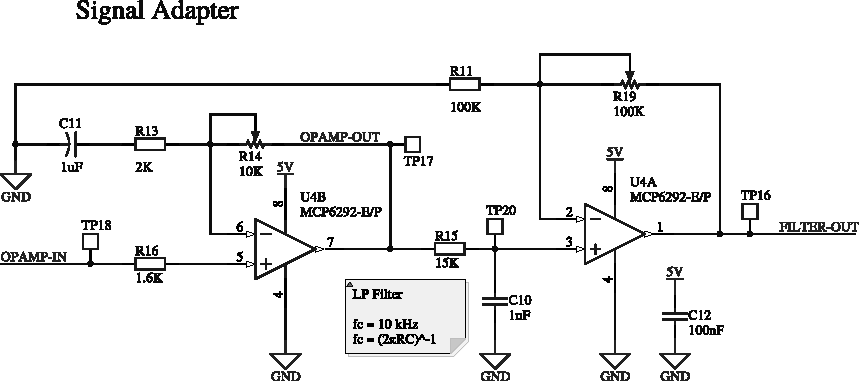
\includegraphics[width=\linewidth]{figures/circuits/filter-ampl-v2}
    \end{figure}
\end{frame}

\begin{frame}{FFT Software}
    L'implementazione utilizzata si chiama
    \vfill
    \begin{center}
        \Large Fixed-Point In-Place FFT
    \end{center}
    \vfill
    \begin{description}
        \item [Fixed-Point] Il numero di bit per la mantissa e per
            l'esponente del valore floating point sono costanti
        \item [In-Place] I risultati sovrascrivono i dati di partenza
        \item [FFT] Fast Fourier Transform
    \end{description}
\end{frame}

\begin{frame}{Software}
    \begin{figure} \centering
        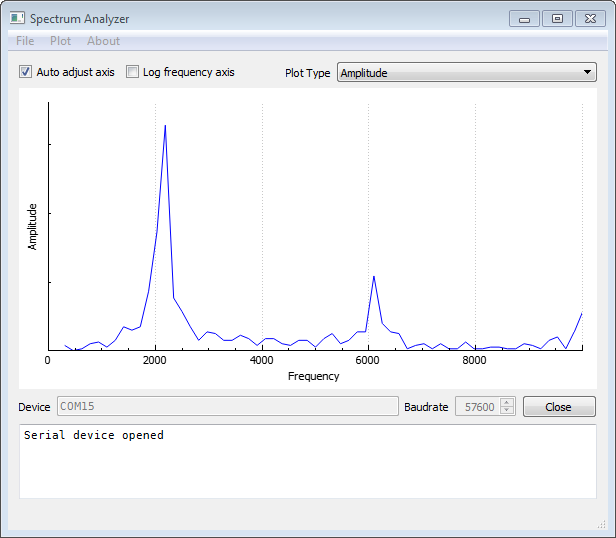
\includegraphics[height=6cm]{figures/screenshots/desktop-windows7-square}
    \end{figure}
    \begin{center}
        \LARGE Demo!
    \end{center}
\end{frame}

\section{Conclusioni}
\begin{frame}{Obiettivi}
    \begin{block}{Raggiungi}
    \begin{itemize}
        \item Analisi spettrale fino a 10\,kHz
        \item Visualizzazione al PC\(^\dagger\)
        \item Esportare immagini / dati
    \end{itemize}
    \end{block}
    \pause

    \begin{block}{Incompleti}
    \begin{itemize}
        \item \(^\dagger\) Visualizzazione delle curve \(\Re(z)\) e \(\Im(z)\) in un solo grafico
        \item Visualizzazione mediante la matrice LED
    \end{itemize}
    \end{block}
\end{frame}

\begin{frame}{Conclusioni}
    \begin{block}{Possibili sviluppi futuri}
        \begin{itemize}
            \item Supporto multipiattaforma
            \item Cronologia spettrale
        \end{itemize}
    \end{block}
    
    \pause
    \begin{center}
        \Large Grazie per l'attenzione
    \end{center}
\end{frame}
 
\end{document}
